\section{Fabrication} \label{sec:fab}

In order to successfully identify the 2 ns electron beam bunch structure delivered by the CEBAF to within 99\% accuracy, the \gx{} Start Counter time resolution is required to be $<350\ \mathrm{ps}$.  In the following section the details of polishing and characterizing machined scintillators, as well as the construction of the Start Counter are discussed.

\subsection{Polishing Machined Scintillators} \label{sec:fab_polish}

The surfaces of the machined scintillators incurred a plethora of surface defects and chemical contaminants known to harm scintillator surfaces while undergoing edge polishing at McNeil Enterprises.  Therefore, in an effort to recover the performance capabilities, polishing was required.

%Prior to polishing the machined scintillators, a coarse measurement of the paddles performance was conducted.
% to understand the magnitude of damage the paddles had incurred, relative to prototypes, as a result of mishandling.  
%The time resolution and light output was measured at three precise locations along the length of the scintillators. One measurement was taken in the middle of the straight section, one in the middle of the bend, and one at the tip of the nose. 

%Figure~\ref{fig:Initial_Paddle_Prop_UW} illustrates the erratic fluctuation and poor performance that existed from paddle to paddle prior to polishing. 
%	\begin{figure}[!htb]
%		\centering
%		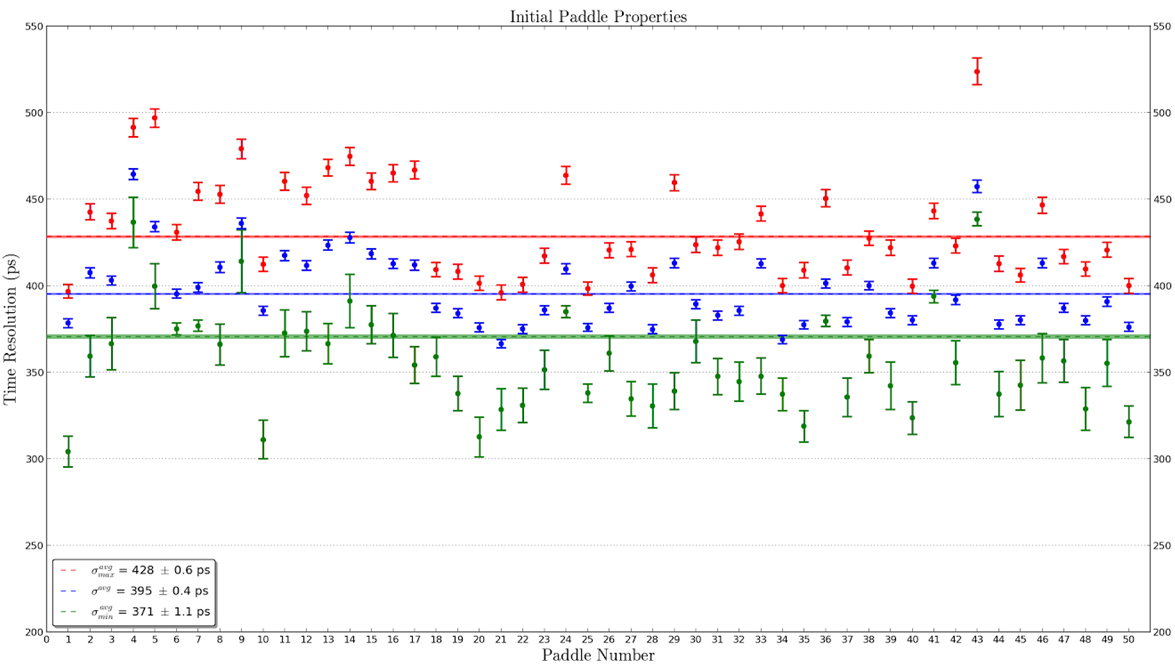
\includegraphics[width=1.0\columnwidth]{fabrication/figs/Initial_Paddle_Prop_UW}
%		\caption{Coarse time resolution measurements prior to polishing. Paddle number is on the x-axis and time resolution in ns is on the y-axis. The red points are the resolutions in the bend region, the blue points are the weighted average of the three measurements, and the green points are the resolutions at the tip of the nose.  The horizontal lines are the weighted averages of the individual measurements.}
%		\label{fig:Initial_Paddle_Prop_UW}
%	\end{figure}
%On average the 50 paddles did not meet the design resolution of 350 ps.

To polish the machined scintillator surfaces, Buehler Micropolish II deagglomerated $\mathrm{0.3\ \mu m}$ alumina suspension was utilized \cite{buehler}.  The polishing suspension was diluted with a 5:1 ratio of de-ionized $\mathrm{H_{2}O}$ to alumina and applied to a cold, wet $6'' \times 0.5''$ Caswell Canton flannel buffing wheel \cite{caswell} operated at $\mathrm{<1500~RPMs}$. All surfaces of the scintillators were carefully buffed until all large, uniform surface defects were removed. In order to eliminate small, localized surface defects hand polishing with a soft NOVUS premium Polish Mate microfilament cloth \cite{novus} and diluted polishing suspension was applied.  These polishing procedures made the scintillators void of virtually all scratches and surface defects.

Once the appropriate polishing procedures had been developed and implemented the surface quality was greatly improved as can be seen in Fig.~\ref{fig:polshing_effects} which illustrates the same scintillator paddle before and after polishing.
	\begin{figure}[!htb]
		\centering
		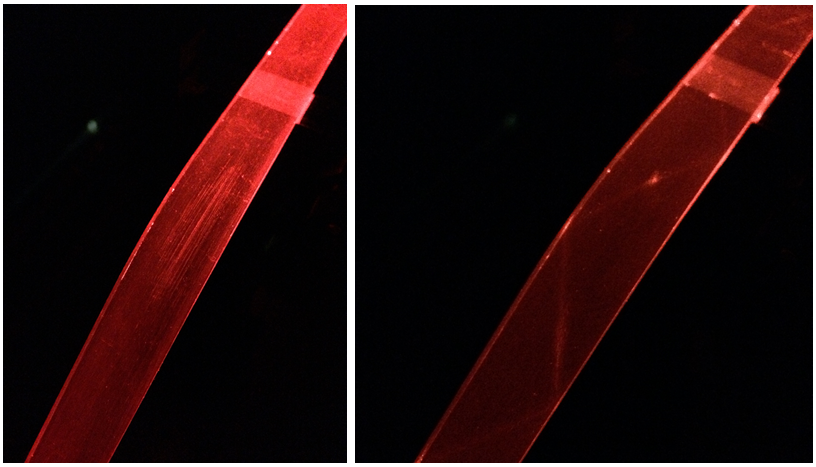
\includegraphics[width=1.0\columnwidth]{fabrication/figs/polshing_effects}
		\caption{Effects of polishing scintillators. Left: non-diffuse laser incident on an edge, before polishing, at the upstream end of the straight section. Right: non-diffuse laser incident on the same edge, after polishing, at the upstream end of the straight section.}
		\label{fig:polshing_effects}
	\end{figure}
A red laser beam was shone into the scintillator medium from the upstream end aimed at one edge so that the total internal reflection towards the tip of the nose was visible.  The unpolished scintillator had such poor surface quality that the reflections in the bend region could not be seen due to the multiple scattering of light at the scintillator boundaries.  However, the reflections in the polished scintillator can clearly be seen traversing down through the nose region.  On average, at the tip of the nose, the scintillators exhibited a $\approx15\%$ improvement in time resolution.  Moreover, a substantial reduction in erratic fluctuations in performance was observed.

%Once the scintillators were polished, their performance was remeasured so that a quantitative measure of the polishing effects were understood.  The measurements were performed in an identical manner outlined above and the pre-polished results were illustrated in Fig.~\ref{fig:Initial_Paddle_Prop_UW}. As expected, the time resolutions were improved as seen in Fig.~\ref{fig:Polished_Paddle_Prop_UW}.
%	\begin{figure}[!htb]
%		\centering
%		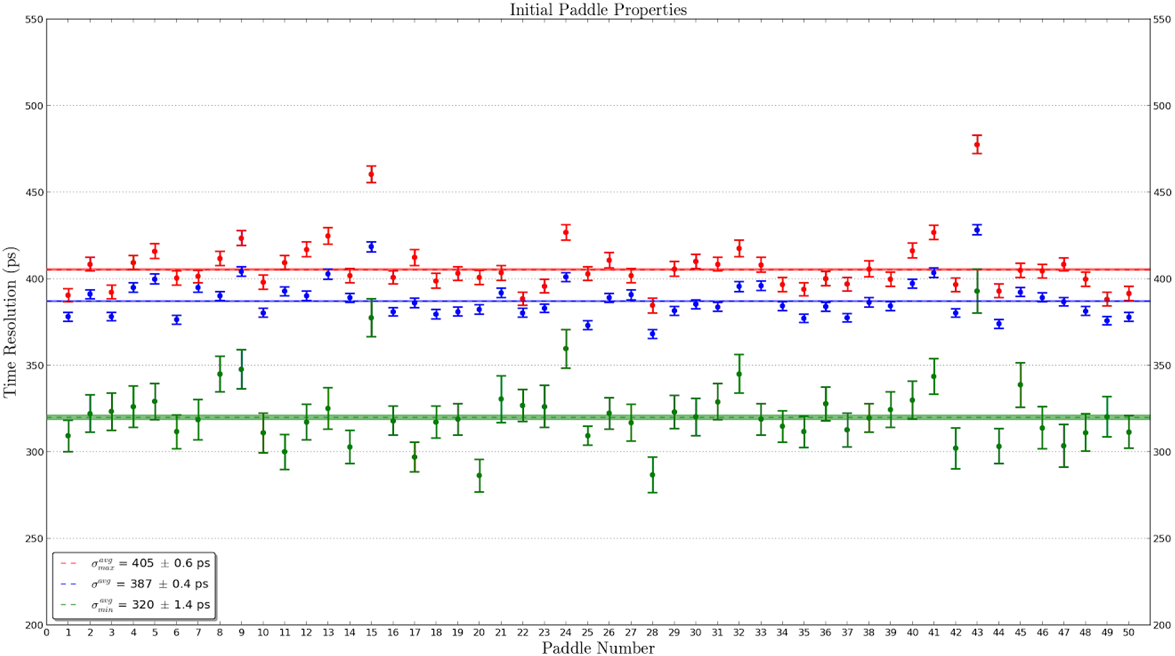
\includegraphics[width=1.0\columnwidth]{fabrication/figs/Polished_Paddle_Prop_UW}
%		\caption{Coarse time resolution measurements after polishing. The details are identical to Fig.~\ref{fig:Initial_Paddle_Prop_UW}}
%		\label{fig:Polished_Paddle_Prop_UW}
%	\end{figure}
%On average, at the tip of the nose, the scintillators exhibited a $\approx15\%$ improvement in time resolution.  Moreover, there was a substantial reduction in erratic fluctuations in performance.

\subsection{Testing} \label{sec:fab_test}

The polished scintillators were tested in order to determine their light output and time resolution properties.  They were measured in an identical and reproducible manner utilizing a custom fabricated test stand shown in Fig.~\ref{fig:test_stand_model}. 
	\begin{figure}[!htb]
		\centering
		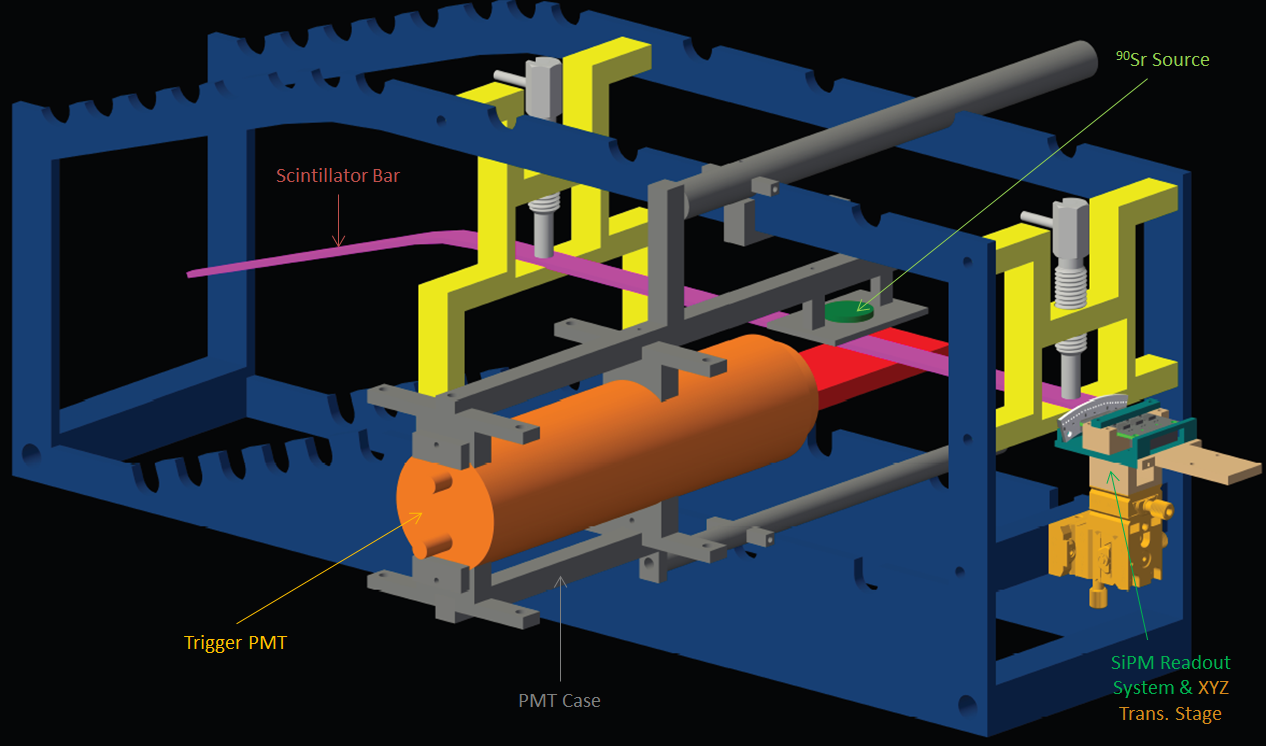
\includegraphics[width=1.0\columnwidth]{fabrication/figs/test_stand_model}
		\caption{CAD Drawing of custom test stand.}
		\label{fig:test_stand_model}
	\end{figure}
The test stand facilitated the precise measurement of the aforementioned scintillator properties at 12 well-defined locations (blue) along the length of the scintillator paddles.  Specifically 4 locations in the straight section, 3 in the bend, and 5 in the nose were tested.  

The measurements were conducted with a collimated $\mathrm{^{90}Sr}$ source (green) oriented orthogonal to the wide flat surface of the scintillators.  The $\mathrm{^{90}Sr}$ source provided minimum ionizing electrons ranging in energy from $\mathrm{0.5-2.3~MeV}$ \textit{via} beta-decay \cite{nndc_sr90}\cite{nndc_y90}.  A trigger photo-multiplier tube (PMT, orange) was placed underneath the scintillator (magenta) on the opposite side of the $\mathrm{^{90}Sr}$ source and provided the TDC start time and ADC gate.  A SiPM detector array (gray) identical to the ones installed in the final ST assembly, was used for readout.  

%The signals from the SiPM and the trigger PMT were then recorded in our data acquisition computer configured with the CEBAF on-line data acquisition (CODA) software.  The signal processing electronics diagram is illustrated in Fig.~\ref{fig:nimelectronicsdiagram}.
%% WB I am not sure we need this here as it is pretty standard
%% EP done.
%	\begin{figure}[!htb]
%		\centering
%		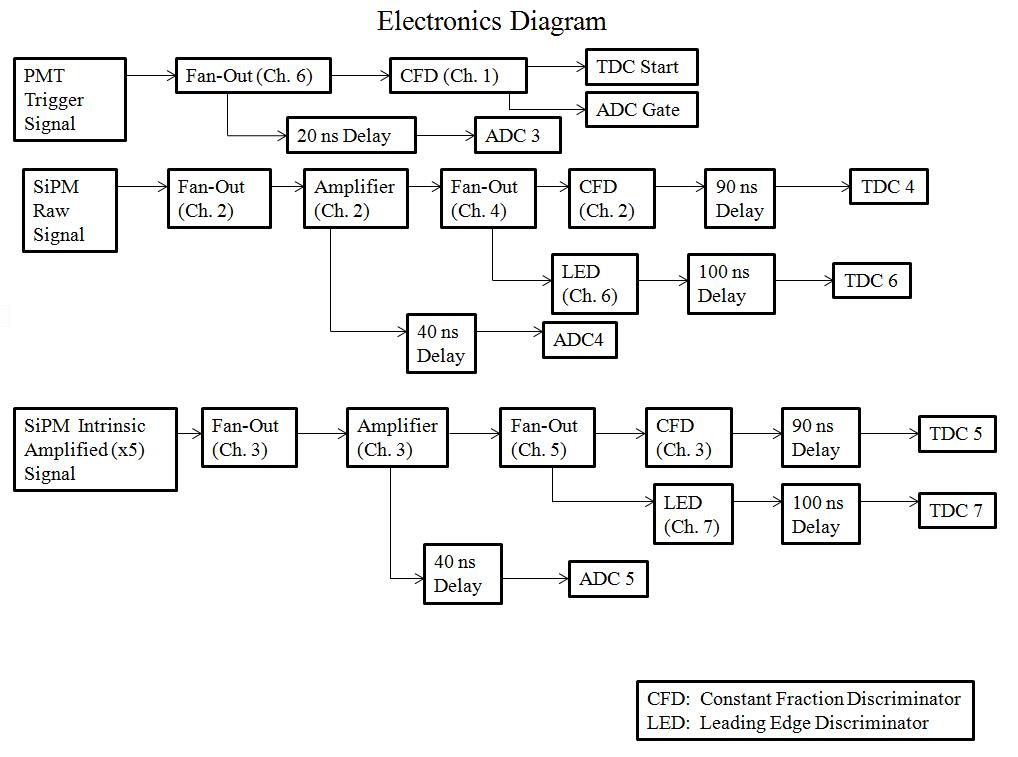
\includegraphics[width=1.0\columnwidth]{fabrication/figs/nim_electronics_diagram}
%		\caption{Electronics diagram for testing machined scintillators.}
%		\label{fig:nimelectronicsdiagram}
%	\end{figure}
The signals from the SiPM and the trigger PMT were then recorded in our data acquisition computer configured with the CEBAF on-line data acquisition (CODA) software.  10,000 event triggers and associated data were collected at each of the locations along the scintillator path.  Subsequently, the ADC and TDC data were analyzed to measure the light output and time resolutions respectively of the whole lot of polished machined scintillators.  

Once the 30 machined scintillator paddles which exhibited the best time resolution and light output properties from the lot of 50 were selected, they were carefully wrapped in Reynolds food grade aluminum foil.  The aluminum foil is $\mathrm{16.5~\mu m}$ thick and possesses good reflectivity properties.  Moreover, the aluminum foil protects the surfaces of the scintillators during both the testing and assembly processes.
  
The measured time resolutions for the 30 best scintillators, which comprise the ST, were found to be satisfactory and even well below design resolution in the nose region which is illustrated in Fig.~\ref{fig:time_res_comp_final_30}.
%	\begin{figure}[!htb]
%		\centering
%		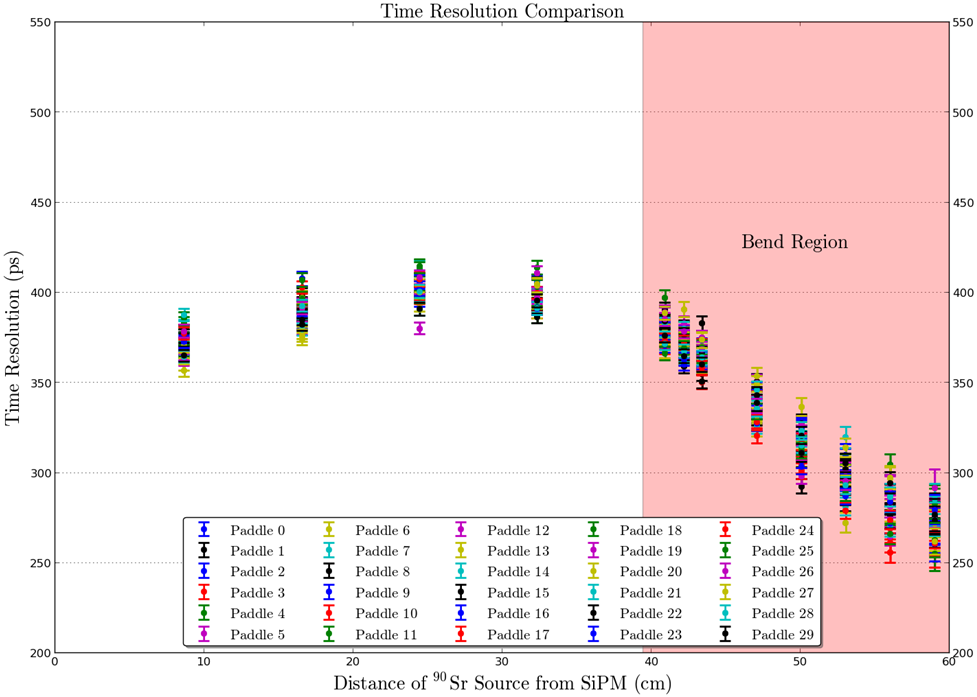
\includegraphics[width=1.0\columnwidth]{fabrication/figs/time_res_comp_final_30}
%		\caption{Time resolution of 30 the best scintillator paddles.  The time resolution performance of the selected scintillators is remarkably similar while illustrating a spread of $\approx 50\ ps$ in the nose region.}
%		\label{fig:time_res_comp_final_30}
%	\end{figure}
	\begin{figure}[!htb]
	\centering
	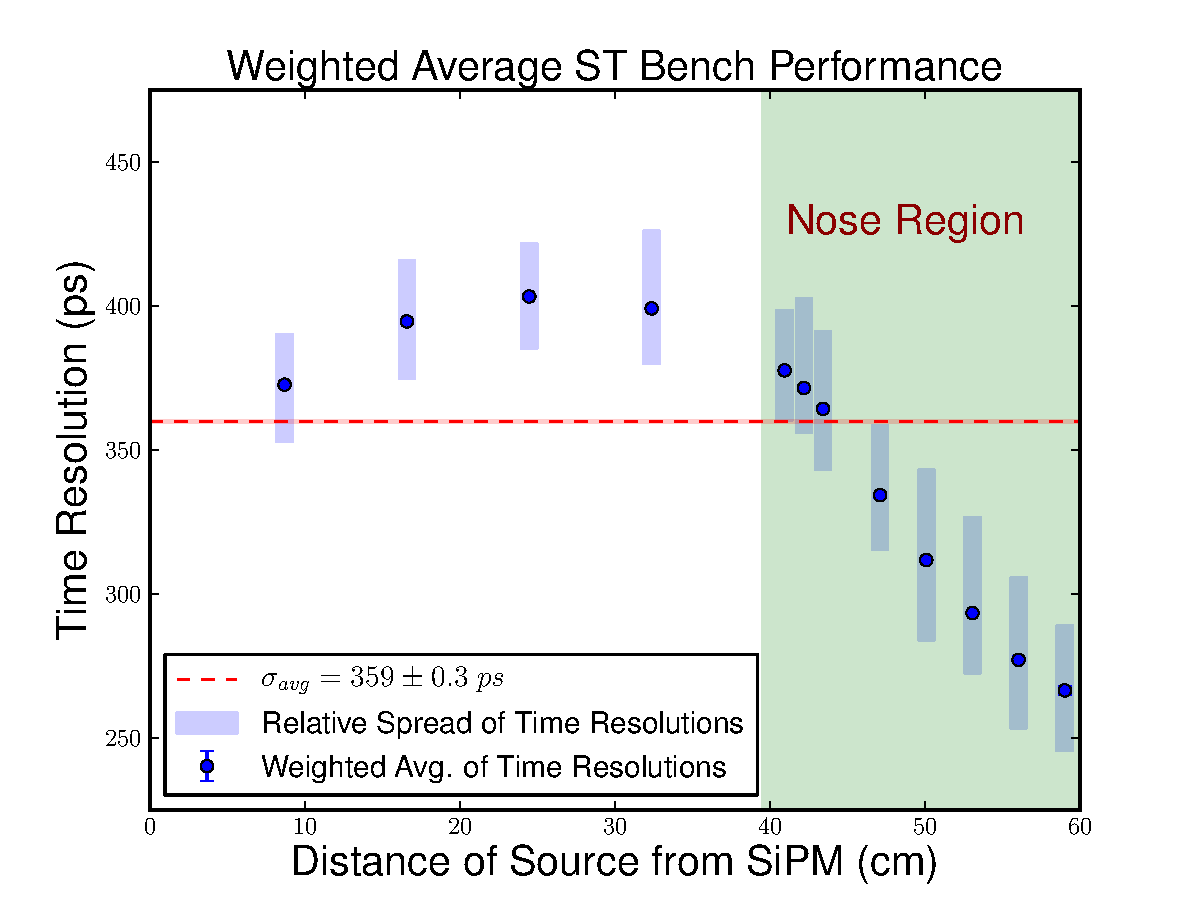
\includegraphics[width=1.0\columnwidth]{fabrication/figs/wtr_vs_dist}
	\caption{Weighted average of the time resolution of 30 the best scintillator paddles versus the source distance from the SiPM as measured on the bench.  The shaded vertical blue boxes indicate the relative spread of the time resolutions among each of the 30 paddles.  The dashed line indicates the weighted average of all 30 paddles for all 12 data points collected for each paddle.  The shaded red horizontal red box indicates the error of the total weighted average.  These paddles were used in the fabrication of the Start Counter.}
	\label{fig:time_res_comp_final_30}
	\end{figure}

The unique geometry of the machined scintillator paddles exhibit a phenomenon of an increase in light collection in the nose region as the light source moves towards the tip at the downstream end.  It is hypothesized that the relatively poor time resolution in the straight section is due to a reflective smearing effect in which light is able to traverse from the straight section down to the tip of the nose, and then back up to the upstream end.

%The average time resolution of the individual scintillators selected for the final ST assembly are shown in Fig.~\ref{fig:final_30_tr_wrapped}.
%	\begin{figure}[!htb]
%		\centering
%		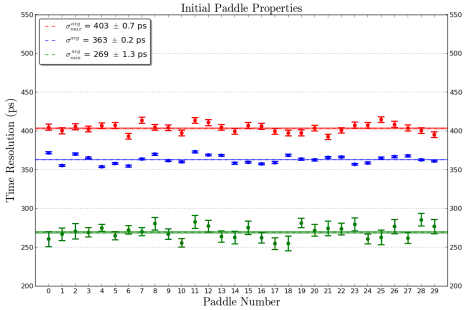
\includegraphics[width=1.0\columnwidth]{fabrication//figs/final_30_tr_wrapped}
%		\caption{Average time resolution of 30 best scintillator paddles.  The red data points correspond to the maximum time resolution obtained in all 12 data points. The blue data points are the weighted average of all 12 data points.  The green data points indicate the minimum time resolution obtained in all 12 data points.}
%		\label{fig:final_30_tr_wrapped}
%	\end{figure}

\subsection{Assembly} \label{sec:fab_ass}

% WB we need a better drawing here
% EP I do not have one
In order to assemble the ST an assembly jig, illustrated in Fig~\ref{fig:ajcaddrawing}, was fabricated.  
	\begin{figure}[!htb]
		\centering
		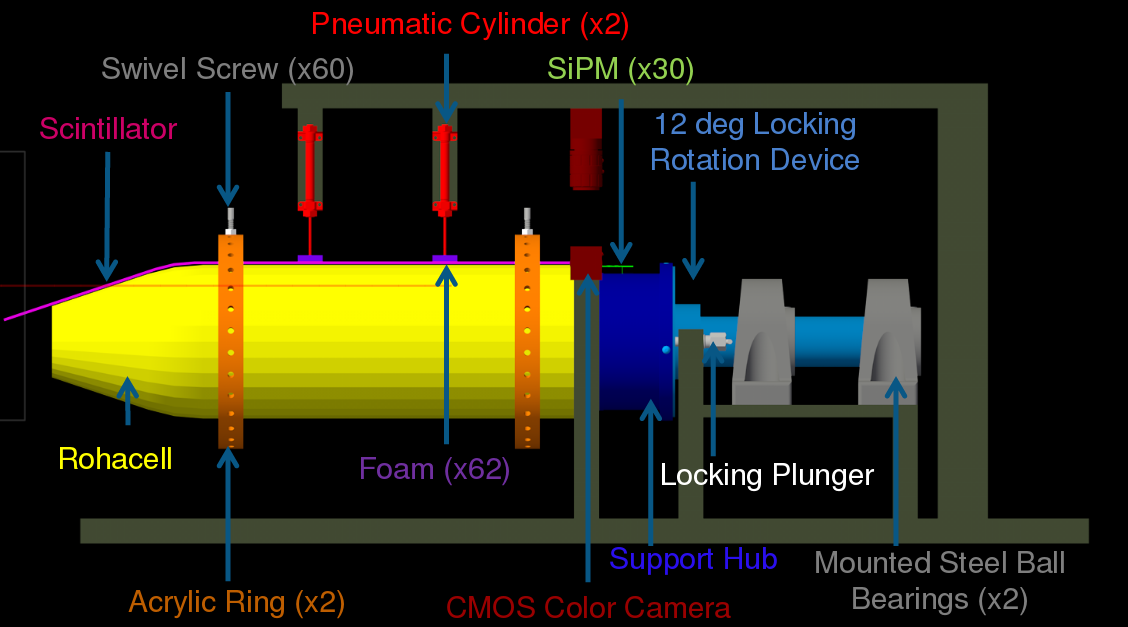
\includegraphics[width=1.0\columnwidth]{fabrication/figs/aj_cad_drawing}
		\caption{CAD drawing of the ST assembly jig.}
		\label{fig:ajcaddrawing}
	\end{figure}
% references to the drawing are needed here suchas :
% consisted of a rotating cylindrical mounting bracket(a) rigidly attached to a 2'' diameter shaft (b) etc. ...
% EP done.
The jig consisted of a rotating cylindrical mounting bracket (light-blue) rigidly attached to a 2'' diameter shaft (light-blue) housed in two cast iron mounted steel ball bearings (gray).  The rotating bracket was engineered such that it was free to rotate unless engaged by a spring loaded locking plunger (light-gray) which would cause the assembly jig to move in discretized $12^{\circ}$ intervals.  This provided the ability to orient paddles (magenta) parallel to the table top so that alignment and coupling could be performed reliably and reproducibly.

While mounted to the assembly jig, the upstream chassis (dark-blue) and Rohacell (yellow) was attached to the rotating bracket.  A vertical bar (dark-green) running parallel to the table above the Rohacell served as a mount for the pneumatic cylinders (red) so that the scintillators could be held firmly in place during installation.  Furthermore, it provided a surface in which a portable flex arm could hold a machine vision camera (dark-red) to monitor the coupling of the scintillators and SiPMs.

A pressurized gas system was implemented to provide manual control of the two pneumatic cylinders with soft, semi-dense rubber feet (purple) attached to the ends.  The rubber feet would hold the scintillator being installed firmly in place by activating two switches which controlled each pneumatic cylinder independently \textit{via} bi-directional solenoids connected in a 5 psi nitrogen gas system.

Two free floating acrylic rings (orange), with 30 tapped holes $12^{\circ}$ apart, were fabricated so as to firmly hold the scintillator paddles in place during assembly. 
%	\begin{figure}[!htb]
%		\centering
%		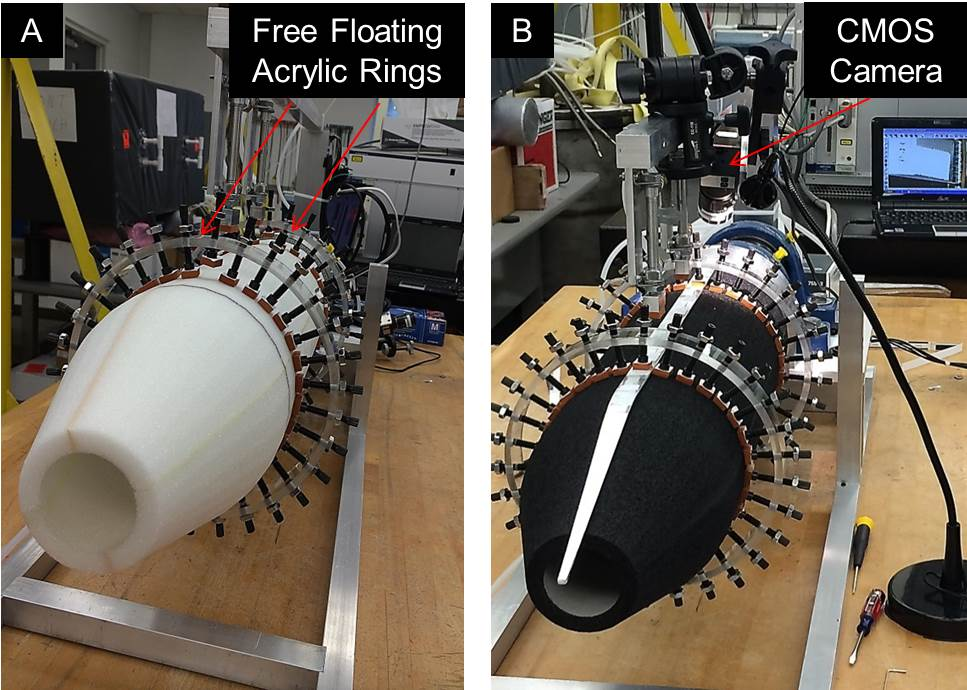
\includegraphics[width=1.0\columnwidth]{fabrication/figs/st_assembly}
%		\caption{Free floating acrylic rings.  Left: Rohacell prior to being painted with black latex paint. Each free floating ring is supported by 30 swivel pad screws. Right: Rohacell after being painted black.  One wrapped scintillator paddled is being held firmly in place by two swivel pad screws.}
%		\label{fig:free_floating_rings}
%	\end{figure}
Each tapped hole housed a $10^{\circ}$ swivel pad thumb screw (light gray) which had silicone foam foot $(0.25 \times 0.25\ \mathrm{in^{2}})$ adhered to it in order to provide a soft barrier between swivel pad and the scintillator surface. 

The camera, seen in Fig.~\ref{fig:aligning_st1_to_hub}, and its associated software were utilized to both measure and control the scintillator/SiPM coupling distances as well as the shimming heights with a precision of $\mathrm{< 10\ \mu m}$ in real time. 
	\begin{figure}[!htb]
		\centering
		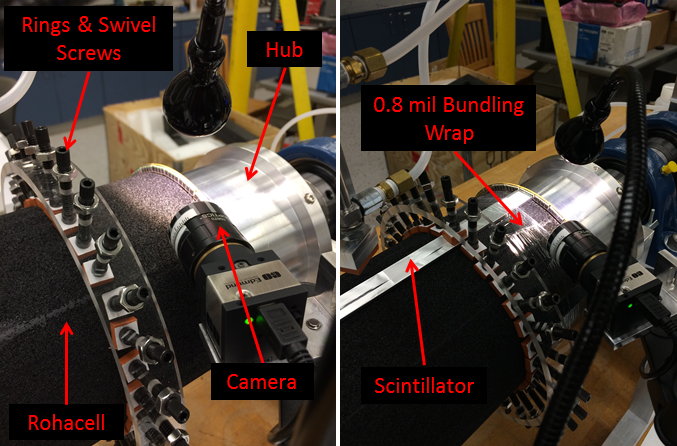
\includegraphics[width=1.0\columnwidth]{fabrication/figs/aligning_st1_to_hub}
		\caption{Aligning ST1 to support hub.  Left: CMOS camera and lamp prepared to monitor ST1 positioning.  Right: Reference scintillator wrapped to Rohacell during ST1 alignment.}
		\label{fig:aligning_st1_to_hub}
	\end{figure}
The camera was calibrated such that at various magnification settings the distance to pixel ratio was known.  The 10 ST1 boards were mounted to the pre-fixed tapped holes along the lip of the upstream support hub.  Black 1 mm spacers were installed between the ST1 PCB and the support hub to avoid any possibility of the electrical contact between the two.  The position of the ST1 was adjusted such that the distance between the top edge of the scintillator and the top edge of the active area of the SiPM was offset by 30 mils ($\mathrm{762\ \mu m}$).  %The offset was measured with the CMOS camera. 

% you do not provide detailed mounting instructions here just the results and parameters

%Each scintillator paddle was carefully installed such that a quantitative measure of the coupling distance and amount of radial shimming required was determined with a high degree of precision and is illustrated in Fig.~\ref{fig:aligning_st1_to_hub}. 

On average each paddle required 30~mils of Kapton polyimide heavy duty film (type HN, $\rho = 1.42\ \mathrm{g/cm^{3}}$) radial shimming.  Moreover, the scintillators were coupled to the SiPM's at a distance of $\mathrm{<\ 200\ \mu m}$.  More details regarding the assembly process are discussed in Ref.~\cite{pooser16}.

%The paddle being installed was carefully positioned such that the upstream end was located approximately a millimeter away (downstream) from the active area of the SiPM and were held in place as seen in Fig.~\ref{fig:aligning_st1_to_hub}. 
%A piece of 0.8~mil bundling wrap was wrapped firmly around the scintillator and the Rohacell structure as seen in Fig.~\ref{fig:aligning_st1_to_hub}. 
% WB pictures can be reduced here
% EP done.

%The distance between the top edge of the scintillator and the top edge of the active area of the SiPM was then measured in order to determine the amount of shimming necessary for radial alignment as illustrated in Fig.~\ref{fig:shimming_effects}. 
%	\begin{figure}[!htb]
%		\centering
%		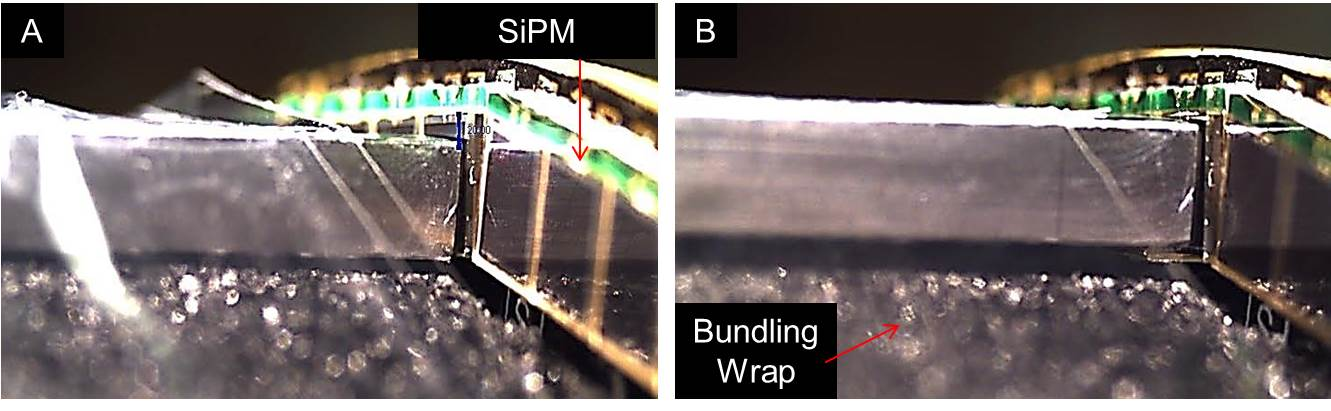
\includegraphics[width=1.0\columnwidth]{fabrication/figs/st_va}
%		\caption[Shimming effects]{Shimming effects.  Left: Before and Right: after shimming.}
%		\label{fig:shimming_effects}
%	\end{figure}
%Three different thickness's (5, 10, 20 mil) of Kapton polyimide heavy duty film (type HN, $\rho = 1.42\ \mathrm{g/cm^{3}}$) were cut into $\mathrm{0.5 \times 12\ in^{2}}$ strips and utilized for shimming the scintillators in the radial direction.  On average, each paddle required 30~mils of radial shimming.

%With the appropriate shimming in place, the paddle was carefully positioned such that the center of the upstream paddle was aligned with the center of the SIPM and the swivel screws were extended.  A piece of computer paper sandwiched between two pieces of Al foil ($\approx 150\ \mathrm{\mu m}$ thick) was then placed parallel to the active are of the SiPM and the paddle was then pressed firmly against the outer most piece of Al foil which is seen in Fig.~\ref{fig:sipm_coupling}.
% WB Pcitures are not necessary here may be a schematic drawing
%	\begin{figure}[!htb]
%		\centering
%		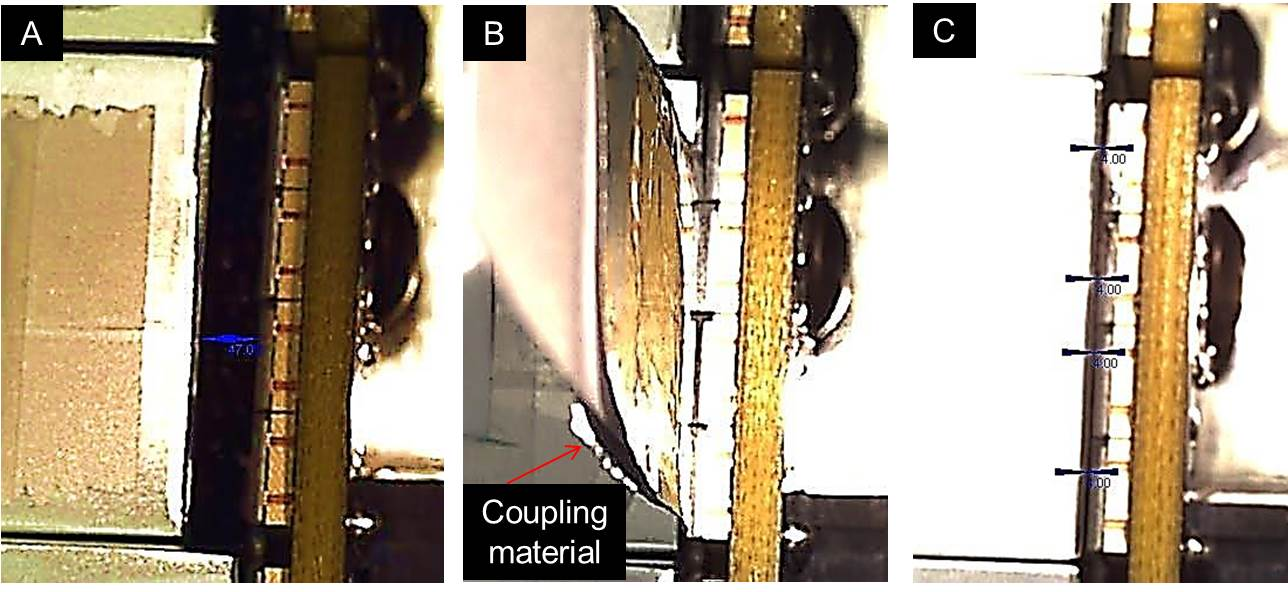
\includegraphics[width=1.0\columnwidth]{fabrication/figs/st_coupling}
%		\caption{Steps of coupling paddles to SiPM.  Left: Paddle prior to being coupled to SiPM.  Center:  Paddle pressed firmly against spacing material and SiPM.  Right: Paddle properly coupled to SiPM at a distance of $162\ \mu m$.}
%		\label{fig:sipm_coupling}
%	\end{figure}
%The piece of computer paper was carefully removed. Then, the Al foil pieces were removed individually so as to ensure no damage was incurred on the paddle surface or SiPM.  Utilizing this method provided a coupling distance $\mathrm{<\ 200\ \mu m}$.

In order to make the ST light tight, an inner cone of black Tedlar polyvinyl fluoride $\rho \approx 1.5\ \mathrm{g/cm^{3}}$ \cite{tedlar_pvf} was taped to the Rohacell as seen in Fig.~\ref{fig:light_tightening_cone}. 
\begin{figure}[!htb]
	\centering
	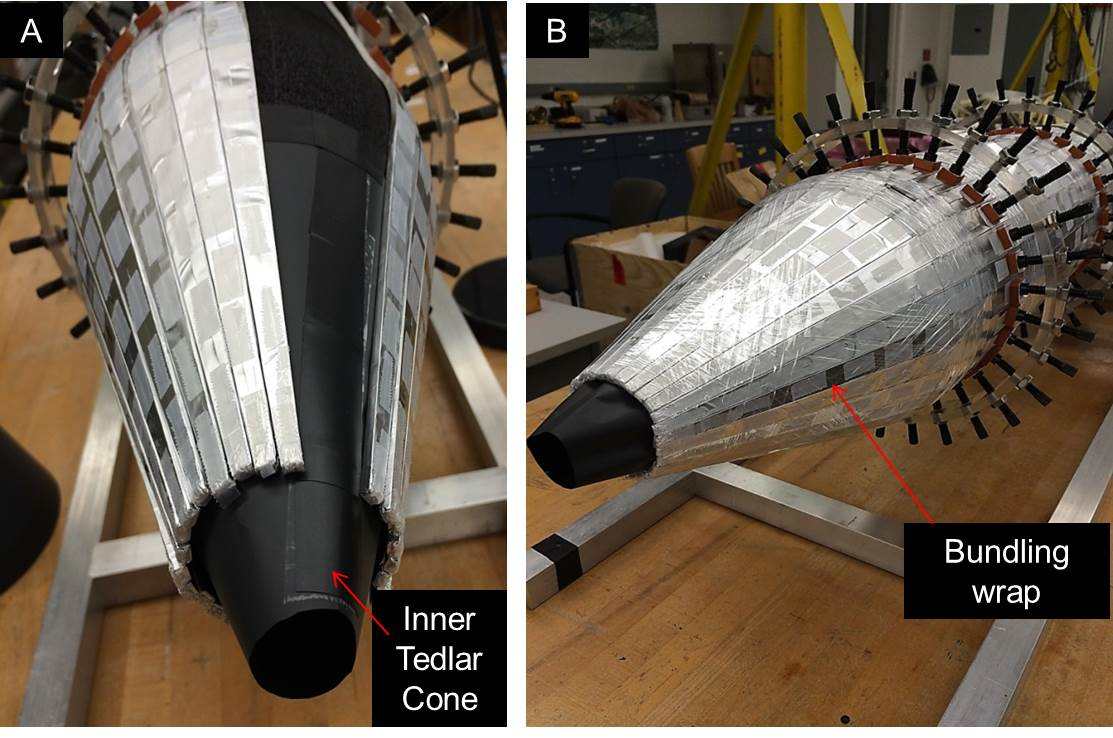
\includegraphics[width=1.0\columnwidth]{fabrication/figs/st_lt_ic_bw}
	\caption{Inner Tedlar cone.  Shown is before and after wrapping with bundling wrap.  The cone was specifically engineered to have the same dimensions of the Rohacell support structure to avoid crumpling of the light tightening material.}
	\label{fig:light_tightening_cone}
\end{figure}
A few gaps existed in the Rohacell at the glue joints, and were filled in with black RTV silicone caulking. Moreover, it was painted with black latex paint for light tightening purposes.  The support hub was also was wrapped with Tedlar and taped down with black electrical tape. The spacing between the ST1 PCBs along with the bottom side of the support hub, was filled with RTV black opaque silicone caulking.  Similarly, RTV silicone caulking was then applied to the inner edge of the collar which encompassed the ST1 PCBs at their outer diameter.

In order to secure paddles to the Rohacell support structure the Start Counter was wrapped along its length using self-adhesive transparent bundling wrap (0.8 mil thick, 6 in wide) at six different locations perpendicular to the central axis of rotation. Four locations were wrapped along the straight section at equal distance $(\approx 8\ \mathrm{cm})$ from one another, one in the bend and one in the nose section.  Five layers of bundling wrap were applied to each section.% and the acrylic rings were removed as illustrated in Fig.~\ref{fig:st_iso_eel}.
% WB only one picture here but with indicators where the bundling wrap sits
%\begin{figure}[tbph]
%	\centering
%	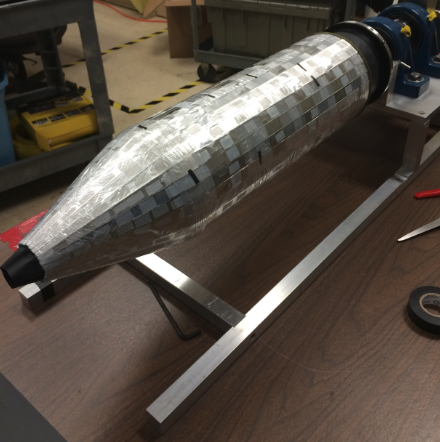
\includegraphics[width=0.8\columnwidth]{fabrication/figs/st_iso_eel}
%	\caption[Isometric view of assembled Start Counter]{Isometric view of assembled Start Counter. The pieces are black electrical tape which mark the ends of bundling wrap are clearly visible.}
%	\label{fig:st_iso_eel}
%\end{figure}

A cone of Tedlar was wrapped around the nose region and taped down with electrical tape as seen in Fig.~\ref{fig:light_tight_st}. 
\begin{figure}[!htb]
	\centering
	\includegraphics[width=1.0\columnwidth]{fabrication/figs/st_lt_v2}
	\caption{Light tight Start Counter mounted to the \gx{} liquid $\mathrm{H_{2}}$ target.  The beam direction is from right to left.  During operation the ST resides in the bore of the superconducting solenoid magnet which is visible in the top left corner.}
	\label{fig:light_tight_st}
\end{figure}
The tips of the inner and outer cones in the nose region were then taped together with electrical tape and trimmed of excess material. Furthermore, a cylindrical piece of Tedlar was taped down at the bend region and to the collar covering the ST1 boards.  The fully assembled and cabled ST mounted to the \gx{} liquid $\mathrm{H_{2}}$ target can be seen in Fig.~\ref{fig:light_tight_st}. 